\documentclass[output=paper,colorlinks,citecolor=brown,
% hidelinks,
% showindex
]{langscibook}
\author{Madeline Critchfield\affiliation{University of Georgia} and Camila Lívio\affiliation{University of Georgia}}
\title{Variable concord in two American Romance varieties: Using Brazilian Portuguese to inform Mosquito Coast Spanish data}
\abstract{In this paper we explore a case of variable number agreement between subjects and verbs found in an under-documented American Romance variety: Mosquito Coast Spanish (MCS). We draw on the literature from Brazilian Portuguese (BP), in which a similar phenomenon has been attested, to guide our analysis. We look at four factors that have proven to be significant in motivating the lack of number concord in BP and find that three of the four: subject/verb word order, presence of intervening material, and high phonic salience of the verb, also are significant predictors in our MCS data. Despite differences in the sociohistorical development of these two varieties, we propose that variable number concord in MCS is motivated by similar language-internal factors and by the process of incomplete language acquisition.}

\IfFileExists{../localcommands.tex}{
  \addbibresource{localbibliography.bib}
  \usepackage{langsci-optional}
\usepackage{langsci-gb4e}
\usepackage{langsci-lgr}

\usepackage{listings}
\lstset{basicstyle=\ttfamily,tabsize=2,breaklines=true}

%added by author
% \usepackage{tipa}
\usepackage{multirow}
\graphicspath{{figures/}}
\usepackage{langsci-branding}

  
\newcommand{\sent}{\enumsentence}
\newcommand{\sents}{\eenumsentence}
\let\citeasnoun\citet

\renewcommand{\lsCoverTitleFont}[1]{\sffamily\addfontfeatures{Scale=MatchUppercase}\fontsize{44pt}{16mm}\selectfont #1}
   
  %% hyphenation points for line breaks
%% Normally, automatic hyphenation in LaTeX is very good
%% If a word is mis-hyphenated, add it to this file
%%
%% add information to TeX file before \begin{document} with:
%% %% hyphenation points for line breaks
%% Normally, automatic hyphenation in LaTeX is very good
%% If a word is mis-hyphenated, add it to this file
%%
%% add information to TeX file before \begin{document} with:
%% %% hyphenation points for line breaks
%% Normally, automatic hyphenation in LaTeX is very good
%% If a word is mis-hyphenated, add it to this file
%%
%% add information to TeX file before \begin{document} with:
%% \include{localhyphenation}
\hyphenation{
affri-ca-te
affri-ca-tes
an-no-tated
com-ple-ments
com-po-si-tio-na-li-ty
non-com-po-si-tio-na-li-ty
Gon-zá-lez
out-side
Ri-chárd
se-man-tics
STREU-SLE
Tie-de-mann
}
\hyphenation{
affri-ca-te
affri-ca-tes
an-no-tated
com-ple-ments
com-po-si-tio-na-li-ty
non-com-po-si-tio-na-li-ty
Gon-zá-lez
out-side
Ri-chárd
se-man-tics
STREU-SLE
Tie-de-mann
}
\hyphenation{
affri-ca-te
affri-ca-tes
an-no-tated
com-ple-ments
com-po-si-tio-na-li-ty
non-com-po-si-tio-na-li-ty
Gon-zá-lez
out-side
Ri-chárd
se-man-tics
STREU-SLE
Tie-de-mann
} 
  \togglepaper[1]%%chapternumber
}{}

\begin{document}
\maketitle

\section{Introduction}

Though widely discussed for Brazilian Portuguese (BP) (\citealt{scherre1998variaccao}; \citealt{naro2000variable}; \citealt{scherre2001origens}; \citealt{guy2005questao}; \citealt{lucchesi2009portugues}; \citealt{brandao2012concordancia}; \citealt{scherre2014sociolinguistic}; \citealt{mendes2015variable}), number variation in Spanish verb morphology has been the subject of relatively few studies with some notable exceptions, including Afro-Bolivian Spanish (\citealt{lipski2008a}; \citealt{sessarego2011status}, \citeyear{sessarego2012non}), Dominican Spanish (\citealt{foote2012role}; \citealt{guy2017african}), and Spanish in the U.S. (\citealt{lipski2008c}). In this paper we analyze a case of variable subject/verb number concord, also referred to as number agreement, (\ref{ex:critchfield:1a}--\ref{ex:critchfield:1b})\footnote{The example from \ref{ex:critchfield:1} in MCS taken from our dataset.} found in Mosquito Coast Spanish (MCS), a contact variety of Spanish spoken by Miskitu speakers in Nicaragua.  


\begin{exe} % declares the example environment
    \ex\label{ex:critchfield:1} 
    \begin{xlist} % declares a list of sub-examples
        \ex\label{ex:critchfield:1a}
        \gll    En    cuanto    al    estilo    de    vida,    ellos    viv-ían diferente.\\  
   in    regards    to    style     of     life      they     live-\textsc{pst}.\textsc{3pl}      differently\\
    \glt    `In regards to lifestyle, they lived differently.'\\
        \ex\label{ex:critchfield:1b}
    \gll   Nuestros    ancestros    antes    viv-ía   de la naturaleza.\\
      our ancestors    before   live-\textsc{pst}.\textsc{3sg}      from    the     nature\\
    \glt    `Our ancestors used to live from nature.'
\end{xlist}
\end{exe}


Our analysis draws from literature on subject/verb number concord in BP to inform our predictions for MCS. We argue that while these two American Romance varieties might differ in some aspects of their historical development, the language acquisition processes that took place in the past by both groups of speakers makes them a valuable comparison in the literature on number concord. In addition, BP is one of the languages where subject/verb agreement has been well-established in the literature, providing a solid foundation to guide us as we explore this phenomenon in a relatively undocumented variety of Spanish.


In this paper, we address (i) what language-internal factors are operative in this variation for both languages and (ii) if the variable concord found in MCS is comparable to the well-established number agreement variation attested in BP. Using a predictive approach in our statistical analysis of the data, we show what factors motivate the variation shown in \ref{ex:critchfield:1a}--\ref{ex:critchfield:1b} and how far it has diffused within the verbal system of MCS. We look at phonic salience of the verb, syntactic order (SV \textit{vs.} VS), intervening material between the subject and the verb, and animacy of the subject. The data used for this study is oral in nature and was collected from narratives and interviews with speakers of MCS in Nicaragua.

The results show that variable number concord in the verbal system of MCS is only found with third-person forms in the dataset, specifically in cases of third-person plural (\textsc{3pp}) subjects and their corresponding verb morphology, either third-person singular (\textsc{3ps}) or \textsc{3pp}. We conclude that variable number agreement in MCS could become more widespread both linguistically and socially, as has been attested in BP (\citealt{mendes2015variable}; \citealt{naro2013remodeling}). This conclusion is based on similarities in internal linguistic factors conditioning non-agreement in both varieties, despite differences in the development of each language under the conditions of adult language acquisition and group language shift.

We first provide relevant sociohistorical background information for both BP and MCS. Then, we detail previous research done on subject/verb number agreement in both BP and other varieties of Spanish as a way to motivate our comparison of these two languages. We follow this with a description of the methodology we use in our analysis of the MCS data. Finally, we discuss our results and how BP can be used to make predictions about how this phenomenon will evolve in MCS, as well as how our findings for MCS may help us better understand what happened historically in the development of this phenomenon in BP.

\section{Background}

\subsection{Sociohistorical context}

Despite Brazilian Portuguese and Mosquito Coast Spanish both exhibiting variation in number agreement between subjects and verbs, these two non-standard American Romance varieties have undergone very different processes of language shift. In Brazil, this shift occurred between the sixteenth and twentieth century with speakers of various African and Amerinidian languages who acquired Portuguese; while in Nicaragua, speakers of Miskitu rapidly acquired Spanish beginning in the middle of the twentieth century \citep[238]{naro2000variable}. The sociohistorical context of BP and MCS is pertinent to the current paper because we argue that the phenomenon under investigation is the direct result of group language shift and incomplete second language acquisition in both varieties, despite the differences that exist in regards to how each language evolved.

A diachronic study by \cite{naro2000variable} traces the variable concord prevalent in BP back to European Portuguese, arguing that the nativization process of Portuguese by adult speakers of languages of diverse backgrounds that began with the colonization has possibly accelerated the process \citep[40]{scherre2001origens}. In this view, they argue, we would have to suppose that such a feature existed and came from Portugal, evolving faster in the new territory due to the intense contact between Portuguese speakers and the indigenous population. In this process of Portuguese's change from a non-native to a native language in that particular speech community, we find an optimal locus for variable concord to thrive in a situation of 
``endemic pidginization and adult second language learning that predominated throughout the history of Brazil'' \citep[237]{scherre2010}. The colonization in the beginning of the 1500s and the second language acquisition process that occurred over subsequent centuries has resulted today in what is primarily a monolingual Portuguese-speaking population in Brazil \citep{lucchesi2009portugues}. 


While MCS speakers in Nicaragua also experienced group language shift and second language acquisition, the process involved Spanish and one specific indigneous language. In addition, this phenomenon occurred much more recently and rapidly in regards to the development of MCS, with the speech community having transitioned from being monolingual Miskitu speakers to bilingual Miskitu-Spanish speakers in the second half of the twentieth century \citep[99]{garcia1996making}. Beginning in the 1950s, the national government implemented the UNESCO sponsored Río Coco Pilot Project for Basic Education, an assimilation program designed to hispanicize the Miskitu people and eradicate ethnic heterogeneity \citep[205--207]{meringer2014accommodating}. A part of this development project involved Spanish-only education along the Caribbean coast, where previously communities were Miskitu-speaking (\citealt[99]{garcia1996making}; \citealt[208]{meringer2014accommodating}). 

The Sandinista Revolution was the impetus for a more constant and robust relationship between the Miskitu speakers from the Caribbean coast and the Spanish speakers from the Pacific. When the Sandinista political party came to power after the Revolution against the national government in the 1970s, a national literacy program was established that promoted the use of the Spanish language \citep[732]{escobar2013}. The Sandinistas wanted to unify the country under a collective identity, similar to the goals of the Río Coco Pilot Project several decades prior \citep[104]{garcia1996making}. One result of this forced linguistic integration attempted by the Sandinistas was the overall community shift toward Spanish as the dominant language in all regions of the country. 

Today, Spanish is considered the official language of Nicaragua and is used as the majority language by the people living on the Pacific coast of the country. Along the northern Caribbean coast, Miskitu, an indigenous language found in Honduras and Nicaragua, is also spoken \citep[721]{catter2011intercultural}. In Nicaragua, the Miskitu-speaking population numbers around 120,000 people, with 91.22\% of these speakers located on the Caribbean coast, geographically isolated from the majority of monolingual Spanish speakers in the country \citep[12]{wilson2012sari}. Along the Caribbean coast, Miskitu and Spanish are spoken on an individual and community level; however, first language Miskitu speakers have slowly begun to shift to Spanish. According to \citet[12--14]{wilson2012sari}, although there is still a strong intergenerational transmission of Miskitu, Spanish is becoming the majority language among the Miskitu community, particularly in the city of Puerto Cabezas, where the data was collected for the current investigation. 

While BP and MCS both represent situations in which adult speakers acquired a second language (due to social or political pressure), there are a number of differences between the cases of these two American Romance varieties, including the types of languages involved, the current bilingual status of the speech communities, and the century and duration of language shift. Despite these sociohistorical differences in their respective developments, both exhibit similar cases of subject/verb non-agreement.

\subsection{Variable concord in Brazilian Portuguese}

There are three contexts in which variable agreement has been attested in spoken (referred to in the literature as `non-standard') varieties of Brazilian Portuguese: \ref{ex:critchfield:2} variable subject/verb agreement, \ref{ex:critchfield:3} number agreement in the noun phrase, and \ref{ex:critchfield:4} number agreement in the predicate phrase.\footnote{\ref{ex:critchfield:2}--\ref{ex:critchfield:4} are adapted from \citet[235]{naro2000variable}.}


\begin{exe} % declares the example environment
    \ex\label{ex:critchfield:2} 
    \begin{xlist} 
        \ex \label{ex:critchfield:2a}
            \gll Eles ganh-am  demais.\\  
                 they earn-\textsc{prs}.\textsc{3pl} {too much}\\
            \glt `They get too much.'\\
        \ex\label{ex:critchfield:2b}
            \gll  Eles ganh-a demais.\\
                  they earn-\textsc{prs}.\textsc{3sg}  {too much}\\
            \glt  `They get too much.'
\end{xlist}
\end{exe}


\begin{exe} % declares the example environment
    \ex\label{ex:critchfield:3} 
    \begin{xlist} 
        \ex \label{ex:critchfield:3a}
            \gll o-s          fregues-es\\  
                 the-\textsc{pl}    customers-\textsc{pl}\\
            \glt `the customers'\\
        \ex\label{ex:critchfield:3b}
            \gll   a-s  {codorna-$\emptyset$}\\
                 the-\textsc{pl}  {game hen-$\emptyset$}\\
            \glt  `the game hens'
\end{xlist}
\end{exe}



\begin{exe} % declares the example environment
    \ex\label{ex:critchfield:4} 
    \begin{xlist} 
        \ex \label{ex:critchfield:4a}
            \gll A-s  coisa-s (es)t-ão  muito    cara-s.\\  
                 the-\textsc{pl}   thing-\textsc{pl}   be-\textsc{prs}.\textsc{3pl}   very expensive-\textsc{pl}\\
            \glt `Things are very expensive.'\\
        \ex\label{ex:critchfield:4b}
            \gll  A-s coisa-$\emptyset$ (es)tá cara-$\emptyset$.\\
               the-\textsc{pl}   thing-$\emptyset$   be-\textsc{prs}.\textsc{3sg} expensive-$\emptyset$\\
            \glt  `Things are very expensive.'
\end{xlist}
\end{exe}

This phenomenon has been extensively studied in BP, particularly from the variationist sociolinguistic perspective. Previous studies have shown that a number of the factors that influence this variation are language-internal, including phonic salience of the verb, subject-verb syntactic order, intervening material between the subject and the verb, and animacy of the subject (\citealt{naro2000variable}; \citealt{mendes2015variable}). 

In regards to subject/verb number variation in BP, \textsc{3pp} contexts have been the most widely researched \textit{(eles fazem/faz} `they do'); however, 1PP contexts are also gaining more attention (\textit{nós fazemos/faz} `we do') \citep[362]{mendes2015variable}. The variation that occurs in \textsc{3pp} subject/verb agreement mirrors what has been observed in MCS, with \textsc{3sg} verb morphology used with \textsc{3pp} subjects. Given the comparable contextual environment and linguistic outcome, BP is the ideal comparison for the MCS data based on SLA conditions, the nature of the variation, as well as the fact that much of the research on this topic in BP has been done through a variationist perspective. 

This phenomenon in BP, as previously mentioned, has been analyzed from a variationist perspective, making it an ideal comparison for our MCS data.

\subsection{Variable concord in Spanish}

When compared with Portuguese, variable subject/verb number agreement in Spanish has been quite understudied; however, there are varieties in which this linguistic phenomenon has been observed, one notable case being that of Afro-Bolivian Spanish (also referred to as Yungueño Spanish). Lipski (\citeyear{lipski2008a}, \citeyear{lipski2008b}) was one of the first linguists to investigate the grammatical features of this dialect in which he noted the use of \textsc{3sg} verbs as invariant forms for all persons and numbers \ref{ex:critchfield:5}.\footnote{\ref{ex:critchfield:5}--\ref{ex:critchfield:6} are adapted from \citet[107--108]{lipski2008a}}




\begin{exe} % declares the example environment
    \ex\label{ex:critchfield:5} 
    \begin{xlist} 
        \ex \label{ex:critchfield:5a}
            \gll Nojotro    tien-e  jrutita.\\  
                 we         have-\textsc{prs}.\textsc{1sg}   fruit\\
            \glt `We have fruit.'\\
        \ex\label{ex:critchfield:5b}
            \gll  Yo no    conoc-ió       hacienda.\\
               I   no    know-\textsc{pst}.\textsc{1sg}   ranch.\\
            \glt  `I never knew the haciendas.'
\end{xlist}
\end{exe}

Lipski (\citeyear{lipski2008a}, \citeyear{lipski2008b}) suggests that this variety of Spanish displays semi-Creole tendencies based on the use of one verb form for all subjects. He attributes the lack of subject/verb agreement to simplification of the verb morphology system resulting from a previous creole stage that the language passed through, due specifically to contact with African substrate languages. 

A different explanation has been proposed by Sessarego (\citeyear{sessarego2011status}, \citeyear{sessarego2012non}), who suggests that the lack of subject/verb agreement found in Afro-Bolivian Spanish is the ``result of imperfect processes of second language acquisition which were able to crystallize in an environment far from the pressure posed by the linguistic norm and language standardization'' \citep[126]{sessarego2011status}. He attests that this explanation may make more sense due to other second language varieties, and non-standard varieties of Spanish and Portuguese containing similar characteristics without a history of contact with creole languages. Instead Sessarego's theory explains the use of one invariant verb form in Afro-Bolivian Spanish as the result of incomplete acquisition and processing difficulties that L2 learners experience at the syntax/semantics interface.

While our analysis aligns more closely to Sessarego's claim, attributing variable subject/verb number concord in MCS to group language shift from Miskitu to Spanish, the actual phenomenon in Afro-Bolivian Spanish does not reflect what we see in MCS as the variation is only observed with third-person. In addition, no quantitative analysis of this feature has been done for Afro-Bolivian Spanish, making it unsuitable for the variationist comparison of this paper.

In addition to Afro-Bolivian Spanish, \cite{foote2012role} have investigated the lack of subject/verb agreement in Dominican Spanish. This dialect seems to be moving in the direction of a less richly inflected verbal system where the \textsc{3ps} verb form can be used with 1PS, \textsc{3ps}, and \textsc{3pp} subjects \ref{ex:critchfield:6}.\footnote{The example from \ref{ex:critchfield:6} is adapted from \citet[432]{foote2012role}}



\begin{exe} % declares the example environment
    \ex\label{ex:critchfield:6} 
  \gll com-e\\
  eat-\textsc{prs}.\textsc{3sg}\\
 \glt `you eat'; `he/she/it eats'; `they eat'\\
\end{exe}

Speakers of this dialect generally weaken or elide the final consonants \textit{–s} and \textit{–n} from the standard verb morphology, which then results in one form for three different subjects. While final \textit{–s} elision is common in many varieties of Spanish, final \textit{–n} elision is specific to Dominican Spanish \citep[364]{lipskirecuero1996}. This extreme weakening of final consonants results in apparent subject/verb non-agreement. 

While it could be argued that final \textit{–n} elision is responsible for the subject/verb disagreement discussed in this paper for MCS, we can provide clear evidence against this suggestion by looking closer at the data, particularly by examining past tense tokens. Cases of imperfect verb forms are difficult to explain, as they could be the result of either final \textit{–n} elision or the use of the \textsc{3ps} form. If final \textit{–n} elision were the cause, the preterite tense would produce forms such as \textit{llegaro}-$\emptyset$ (instead of \textit{llegaron} `they arrived'); however, this is not the case. While examples like \ref{ex:critchfield:7a}\footnote{The example from \ref{ex:critchfield:7} in MCS taken from our dataset.} could be argued as \textit{–n} elision, examples in the preterite like \ref{ex:critchfield:7b}, do not demonstrate final \textit{–n} elision, but the clear use of \textsc{3ps} verb morphology. Based on this difference in phenomena, Dominican Spanish also does not present an ideal comparison for our MCS data.



\begin{exe} % declares the example environment
    \ex\label{ex:critchfield:7} 
    \begin{xlist} 
        \ex\label{ex:critchfield:7a} 
            \gll Ellos    nunca    aguant-aba       de    nada.\\  
            they    never  tolerate-\textsc{pst}.\textsc{3sg}      of     nothing\\
            \glt `They never tolerated anything.'\\
        \ex\label{ex:critchfield:7b} 
            \gll  Los          miskito-s      dij-o.\\
             the-\textsc{pl}   miskito-\textsc{pl}   	say-\textsc{pst}.\textsc{3sg}\\
            \glt  `The Miskitus said.'
\end{xlist}
\end{exe}


In addition to Afro-Bolivian Spanish and Dominican Spanish, a case of variable subject/verb concord has been identified in bilingual speakers of English and Spanish in the United States (\citealt{lipski1993creoloid}, \citeyear{lipski2008c}). \citet[56]{lipski2008c} categorizes these speakers as transitional bilinguals because their passive linguistic skills are equal to that of a native speaker of Spanish but their active production of the language is slightly less developed than first language Spanish speakers. Transitional bilinguals are usually individuals who spoke Spanish as children but who have become English-dominant with age \citep[56]{lipski2008c}. A notable characteristic of the Spanish spoken by transitional bilinguals in the U.S. is the use of third-person verb morphology for first and second-person subjects, including the use of the \textsc{3ps} verb form \ref{ex:critchfield:8}\footnote{The example from \ref{ex:critchfield:8} is adapted from \citet[59]{lipski2008c}.} in place of the \textsc{3pp} \citep[59]{lipski2008c}.  

\begin{exe} % declares the example environment
    \ex\label{ex:critchfield:8} 
  \gll Vien-e mis tíos.\\
 come-\textsc{prs}.\textsc{3sg} my {aunt and uncle}\\
 \glt `My aunt and uncle come.'\\
\end{exe}

The variation present among transitional bilinguals in the U.S. has been connected to acquisition, attributed to residual competence in Spanish due to either insufficient input in the context of a primarily English-speaking environment or an overall shift toward the majority language of English. While this variety displays non-agreement in \textsc{3pp} contexts, \textsc{3sg} verb forms are also used with other persons and numbers, making it different from what we observe in MCS. Also, in the case of MCS, Spanish is considered the majority language and represents the language speakers are shifting toward, not away from, as is the case for transitional bilinguals in the United States.

\section{Methodology}

The present study draws on oral data collected through sociolinguistic interviews with 10 Mosquito Coast Spanish speakers (see Appendix A for social information on participants). The interviews took place in the city of Puerto Cabezas, Nicaragua during the summer of 2017, where all participants currently reside. The material was recorded and subsequently transcribed by the first author, and later reviewed by a native speaker of  Nicaraguan Spanish. 

All the explicit \textsc{3pp} subjects and their corresponding verbs were extracted from the transcribed data (n=389). The coding was based on previous predictors found to be significant for a similar phenomenon in Brazilian Portuguese \citep{naro2000variable}: phonic salience of the verb (high or low salience), syntactic order of the subject and the verb (SV or VS), the presence of intervening material between the subject and the verb (yes or no), and animacy of the subject ([+human] or [-human]).

In the context of this study phonic salience relates to the number morpheme marked on the verb, referred to as the singular/plural opposition. In BP, lack of agreement occurs more frequently when there is ``a less perceptible difference in form between the singular and plural'' \citep[243]{naro2000variable}. This concept is directly related to tense/mood, with present and imperfect forms being less salient (\textit{come/comem} ‘he/she eats/they eat’), where the difference in forms is solely based on the nasalization of the final vowel. In contrast, preterite forms are considered to be the most salient (\textit{ganhou/ganharam} ‘he/she won/they won’), where there is often a difference in both the root vowel and in the number of syllables \citep[165]{scherre2010}. In MCS, \textsc{3pp} forms that differ from their singular counterpart by only a final nasal consonant were coded as having low phonic salience, (\textit{trabajan vs. trabaja} in \ref{ex:critchfield:9}).\footnote{The example from \ref{ex:critchfield:9} in MCS taken from our dataset.} Forms that contain a larger perceptible distinction between singular and plural (\textit{dijeron vs. dijo} in \ref{ex:critchfield:10})\footnote{The example from \ref{ex:critchfield:10} in MCS taken from our dataset.}, were coded as having high phonic salience.


\begin{exe} % declares the example environment
    \ex\label{ex:critchfield:9} 
    \begin{xlist} 
        \ex \label{ex:critchfield:9a}
            \gll Los hombres   trabaj-an.\\  
            the  men         work-\textsc{prs}.\textsc{3pl}\\
            \glt `The men work.'\\
        \ex\label{ex:critchfield:9b}
            \gll Ellos  trabaj-a   de      la  agricultura.\\
             They  work-\textsc{prs}.\textsc{3sg}    from the  agriculture\\
            \glt  `They work from the agriculture.'
\end{xlist}
\end{exe}


\begin{exe} % declares the example environment
    \ex\label{ex:critchfield:10} 
    \begin{xlist} 
        \ex \label{ex:critchfield:10a}
            \gll Ellos   le      dij-eron             que    no    les        llev-ara.\\  
            they   him    tell-\textsc{pst}.\textsc{3pl}   that    no    them     take-\textsc{pst}.\textsc{sbjv}.\textsc{3sg}\\
            \glt `They told him not to take them.'\\
        \ex\label{ex:critchfield:10b}
            \gll Entonces  los         pajarito-s    dij-o                 que    había         un   techo.\\
            then the.\textsc{pl}   bird-\textsc{pl} say-\textsc{pst}.\textsc{3sg} that  {there was}   a  roof\\
            \glt  `Then the birds said that there was a roof.'
\end{xlist}
\end{exe}

The syntactic order of the subject and the verb also contribute to variable number concord in BP, with VS word order favoring non-agreement \citep[363]{mendes2015variable}. In our analysis, we considered all the cases in which the subject appeared both before and after the verb, with the position of the subject being computed as either preceding \ref{ex:critchfield:11}\footnote{The example from \ref{ex:critchfield:11} in MCS taken from our dataset.} or postposing \ref{ex:critchfield:12}\footnote{The example from \ref{ex:critchfield:12} in MCS taken from our dataset.} the verb. 



\begin{exe} % declares the example environment
    \ex\label{ex:critchfield:11} 
            \gll los    niños      inocentemente le     dij-o\\  
           The  children  innocently       him  tell-\textsc{pst}.\textsc{3sg}\\
            \glt `The children innocently told him.'\\
\end{exe}

\begin{exe}
    \ex\label{ex:critchfield:12}
     \gll Lleg-ó                   los   duendecitos.\\
            arrive-\textsc{pst}.\textsc{3sg}   the   elves\\
            \glt  `The elves arrived.'\\
\end{exe}


Intervening material is another factor proven to be significant in BP (\citealt{naro2000variable}; \citealt{mendes2015variable}), with higher rates of non-agreement occurring when the subject and verb are not located directly next to one another. In our dataset, tokens were coded as having no intervening material when the subject and verb were located next to each other in the utterance and having intervening material if any other element was located between them. Examples of other elements include adverbs \ref{ex:critchfield:13}\footnote{The example from \ref{ex:critchfield:13} in MCS taken from our dataset.} and clitics \ref{ex:critchfield:14}\footnote{ The example from \ref{ex:critchfield:14} in MCS taken from our dataset.}.



\begin{exe} % declares the example environment
    \ex\label{ex:critchfield:13} 
            \gll los mosquitos siempre habl-a\\  
          the.\textsc{pl} Miskitus always speak-\textsc{prs}.\textsc{3sg}\\
            \glt `The Miskitus always talk.'\\
\end{exe}

\begin{exe}
    \ex\label{ex:critchfield:14}
     \gll algunos lo habl-an contando en miskitu y algunos lo habl-a     más rápido\\
     some    it  {speak-\textsc{prs}.\textsc{3pl}}  singing  in Miskitu and some it speak-\textsc{prs}.\textsc{3sg} more fast\\
            \glt  `some speak it singing in Miskitu and some speak it faster.'\\
\end{exe}

Finally, in regards to animacy, subjects that were human were coded as such \ref{ex:critchfield:11}, while subjects that were inanimate were coded as non-human \ref{ex:critchfield:15}\footnote{The example from \ref{ex:critchfield:15} in MCS taken from our dataset.}. In BP, [+human], [+animate] subjects are more likely to result in subject/verb agreement \citep[363]{mendes2015variable}.


\begin{exe}
    \ex\label{ex:critchfield:15}
     \gll Las bebida-s típicas sería chicha. \\
       the.\textsc{pl} drink-\textsc{pl} typical be-COND.\textsc{3sg} chicha\\
            \glt  `The typical drinks would be chicha.'\\
\end{exe}

While variable concord has been studied in other varieties of Spanish (\citealt{lipski2008a}, \citeyear{lipski2008b}; \citealt{sessarego2011status}, \citeyear{sessarego2012non}; \citealt{foote2012role}; \citealt{guy2017african}), we believe that the comparison between MCS and BP is more consistent for several reasons. First, the methodological approaches employed in the studies on Spanish are mostly descriptive, whereas the literature on BP has a comprehensive discussion of the phenomenon from a variationist approach. Furthermore, this context of variation has been vastly discussed and documented in the past 40 years in this variety of Portuguese \citep[358]{mendes2015variable}, which makes it an optimal point of comparison for other typologically similar varieties. Additionally, the nature of the variation in MCS aligns with what we find in BP and both varieties experienced group language shift via second language acquisition, albeit differences in their historical evolution.

The research questions that guide our analysis are the following: 1) What is the overall frequency of non-agreement between subjects and verbs in MCS?, and 2) What are the most predictive factors in this variation context? We hypothesize that the significant variables reported for the same phenomenon in Brazilian Portuguese will have an effect in this variety of Spanish given the typological similarities and the process of second language acquisition and language shift that occurred in both cases. We therefore expect low phonic salience, VS word order, presence of intervening material between subject and verb, and [+human] subjects to favor lack of agreement in MCS \citep{naro2000variable}. 

Our data was subjected to both a logistic regression and mixed-effects logistic regression to model the relationship between the categorical response variable (concord vs. no concord) and all the motivated predictors mentioned above. 

\section{Results and discussion}

\subsection{Analysis of the data}

In our analysis of the Mosquito Coast Spanish data, we specifically look at the variation in number agreement between \textsc{3pp} subjects and their corresponding verbs. Compared to Brazilian Portuguese, where variable number concord occurs in several different contexts, we have only observed cases of variation in subject/verb number agreement in our data. The general frequency results (\figref{fig:critchfield:3}) for this variety of Spanish show that lack of agreement occurs in 20.3\% of the dataset overall (n=79).

\begin{figure}
    
    \includegraphics[scale=0.55]{../figures/critchfield_f1.png}
    \caption{General distribution of the variation}
    \label{fig:critchfield:1}
\end{figure}

Based on the limited context where this variation is found in MCS, it is not surprising that the rate of usage is not as high when compared to BP. However, even among speakers of BP, rates of agreement vary. \citet[362]{mendes2015variable} state that there is great variability among communities in Brazil as far as subject/verb agreement in the \textsc{3pp} goes, ranging from 17\% to 94\%, with rural speakers who possess little formal education displaying higher rates of non-agreement compared to educated urban speakers. This variability is apparent in the various studies done throughout the state of São Paulo, with speakers in the rural zones producing rates of \textsc{3pp} agreement as low as 24\% of the time (see Pereira 2004)\todo{Bibliography entry missing} and speakers in urban zones, such as São José do Rio Preto and the city of São Paulo, producing rates of \textsc{3pp} agreement 73\%  and 87\% of the time respectively (see Rubio and Gonçalves 2012 and \citealt{oushiro2015identidade}). Our findings for MCS are based on one group of speakers, all residing in the city of Puerto Cabezas. It is possible that MCS could reflect the same variability in rates as BP if speakers from both rural and urban areas were included in the analysis. While not within the scope of the current study, this inclusion of speakers from a variety of locations would be interesting to analyze in future studies.

In order to determine what motivates the variation that we observe in our data, we look at four internal language factors that have been attested in the literature on variable concord in BP \citep{naro2000variable}. The regression model\footnote{Concordance index C of the binomial logistic regression is C=0.679. The model presents acceptable discrimination \citep[259]{levshina2015linguistics} .} confirms that several factors have shown predictive power, and that the chances of getting non-agreement between subjects and verbs is 1.06 higher when the phonic salience of the verb is low, the word order is VS, there is intervening material between the subject and the verb, and the subject presents a [+human] feature. Initial plotting of the dependent variable therefore correlates with the trends discussed for BP.

\newpage

\begin{figure}
   \includegraphics[scale=0.40]{../figures/critchfield_Rplot_3.png}
    \caption{General predictor trends}
    \label{fig:critchfield:2}
\end{figure}



Phonic salience of the verb form, the order of the verb in relation to the subject, and intervening material between subject and verb were the three most predictive factors in the model. The only factor that was not significant in the statistical analysis was the animacy of the subject. Based on these results, we observe that similar factors seem to play a role in the number variation between subjects and verbs in both BP and MCS, with the exception of animacy, which could be due to the number of [-human] tokens in the dataset. Of the 389 examples analyzed, only 38 were [-human] and the rest of the tokens were [+human]. The lack of representation of non-human subjects in our data could have led to animacy being statistically insignificant in the analysis. 


\newpage
\begin{table}[]
    
    \begin{tabular}{lrrrr} 
    \lsptoprule
    \textbf{AIC} & \textbf{BIC} & \textbf{logLik} & \textbf{Deviance} & \textbf{df. resid.}\\ 
    \midrule
     363.3 & 387.1 & -175.7 & 351.3 & 383\\ 
    \midrule
    
   \multicolumn{5}{l}{\textbf{Random effects:}}\\ 
     \textbf{Groups} & \textbf{Name} & \textbf{Variance} & \textbf{Std. Dev.} &\\ 
    %  \midrule
     Speaker & (Intercept) & 0.9094 & 0.9536 & \\ 
    \multicolumn{5}{l}{Number of obs: 389, groups: Speaker, 10}\\
    \midrule
    
    \multicolumn{5}{l}{\textbf{Fixed effects:}}\\ 
      & \textbf{Estimate} & \textbf{Std. Error} & \textbf{z value} & \textbf{Pr(>|z|)}\\
    %  \midrule
     (Intercept) & -0.08567 & 0.52902 & -0.162 & 0.87134\\ 
     Order SV & -1.10528 & 0.39076 & -2,829 & 0.00468 **\\ 
     Proximity & -0.55266 & 0.30027 & -1.841 & 0.06569 '\\ 
     Phonic.SalienceHigh & -1.08205 & 0.56114 & -1.928 & 0.05381 '\\ 
     AnimacyNon-Human & 0.43979 & 0.44226 & 0.994 & 0.32002\\ 
    \multicolumn{5}{l}{\textbf{Signif. codes:} \quad 0 `***' 0.001 `**' 0.01 `*' 0.5 `.' 0.1 `{}' 1}\\ 
    \lspbottomrule
    \end{tabular}
    \caption{GLMM predicting variable concord in MCS data}
    \label{tab:critchfield:1}
\end{table}

The syntactic order (SV or VS) is known as a highly significant predictor in BP data (\citealt{guy1981linguistic}; \citealt{naro2000variable}; \citealt{mendes2015variable}). The VS order has proven to have an effect on MCS, favoring the occurrence of non-agreement.



\begin{exe}
    \ex\label{ex:critchfield:16}
     \gll Cuando viene otras personas de otros paises.\\
     {}\\
     \glt  `When other people come from other countries.'\\
\end{exe}

Furthermore, the presence of material between subject and verb also favors lack of agreement, which is another effect of the syntactic order configuration. Finally, phonic salience is described as a highly indicative variable for the presence of variation in the context in question in BP (\citealt{brandao2012concordancia}; \citealt{mendes2015variable}, among many others). What we observe in MCS is that this variable is statistically significant and behaves very similarly to BP: 
``less salient forms favor the absence of plural markers, whereas more salient forms favor the overt realization of the plural morpheme'' \citep[362]{mendes2015variable}. Likewise, our data shows that the lower the phonic salience, the more cases of non-agreement we get, as in \textit{las otras personas que viene de otros países} `the other people that come from different countries', and \textit{las personas del pacifico dice} `people from the Pacific say'. 

In order to conceptualize how MCS compares to BP and standard varieties of Spanish and Portuguese, we created the continuum in \figref{fig:critchfield:3}. Based on the variety of contexts where lack of number concord has diffused in BP, it is located farther along on the continuum as it is more linguistically and socially widespread. On the other end, we find standard varieties of Spanish and Portuguese. Somewhere in the middle is where MCS stands. As demonstrated in our analysis, this variety of Spanish shows variation in number agreement between subjects and verbs, however, it does not seem to have infiltrated other contexts such as the noun phrase or predicate phrase, as in BP. Despite this fact, our analysis also shows that many of the same predictors are at play in the number agreement variation in MCS and in BP.

\begin{figure}

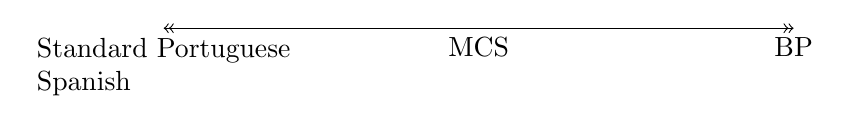
\begin{tikzpicture}
\draw [<<->>]
(0,0) node[align=left,   below] {Standard Portuguese\\Spanish} --
(4,0) node[align=center, below] {MCS}     -- 
(8,0) node[align=right,  below] {BP};
\end{tikzpicture}

    \caption{Continuum of change of inflexional morphology in Romance}
    \label{fig:critchfield:3}
\end{figure}


In addition to showing similar patterns in subject/verb variable concord, BP and MCS both represent cases of non-standard American Romance varieties whose speakers have undergone language shift. The development of a second language via natural second language acquisition and group language shift can result in the incomplete acquisition of some features of the target language (Winford 2003:222)\todo{Bibliography entry missing}. As a result, certain elements of the interlanguage may fossilize, or cease to be acquired in a target-like manner, such as simplification of the verb morphology system. While this is an attested result of second language acquisition, it is impressive that MCS and BP share as many similarities in their predictors of variation as they do, considering the differences in how each language developed historically. 

While we can use BP to predict how this phenomenon will evolve in MCS, we may also be able to use our findings for MCS to better understand what happened historically in the development of this phenomenon in BP. Drawing on uniformitarianism, \citet[161]{labov1972sociolinguistic}  states that we must assume that the same mechanisms involved in past language change are those which we can observe in the present. Therefore, the pattern and context of variation we find for MCS may reflect what this phenomenon first looked like in BP in the beginning of its development.

\section{Conclusions}

In this paper, we have argued that the number agreement variation observed in Mosquito Coast Spanish shows greater correlation with Brazilian Portuguese than with other Spanish varieties for many reasons, including the similarities in the nature and context of the variation and the linguistic factors that predict non-agreement. The results of our statistical analysis for MCS closely align with BP in regards to the linguistic factors that predict the variation of \textsc{3pp} subject/verb number agreement. These findings are particularly impressive because of the differences the varieties demonstrate in their historical evolution via second language acquisition and group language shift. Our results may suggest that variable number concord in MCS could become more widespread both linguistically and socially, as has been attested in BP and may also help us better understand how this phenomenon first evolved in Brazilian Portuguese. 

The current comparison is productive because not only does it provide more evidence of the phenomenon of subject/verb non-agreement in another American Romance variety, but it may also tell us something more about language change, specifically that which occurs when languages come into contact. The fact that many of the language-internal factors that rule subject/verb agreement variation are the same for both varieties, despite the differences regarding their development, reflects possible universal tendencies that occur in language contact scenarios. Future research on this topic in MCS should expand on sociolinguistic factors and include a detailed analysis for all persons and numbers in order to determine if the variation we currently see in MCS reflects what we find for BP. This information will allow us to draw more conclusions about how variation in number agreement may develop in the future for MCS, as well as give us more insight into how this phenomenon first evolved in Brazilian Portuguese.

\newpage
\section*{Appendix}
\begin{table}[]
    
    \begin{tabular}{rlrl} 
    \lsptoprule
    \textbf{Participant} & \textbf{Gender} & \textbf{Age} & \textbf{Level of Education}\\ 
    \midrule
     1 & Female & 20 & Secondary\\ 
     2 & Female & 18 &  Secondary\\ 
     3 & Female & 19 & Secondary\\ 
     4 & Male & 23 & University\\ 
     5 & Male & 25 &  University\\ 
     6 & Male & 52 & University\\ 
     7 & Male & 47 & Secondary\\ 
     8 & Male & 50 & Secondary\\ 
     9 & Male & 40 & University\\ 
     10 & Female & 30 & University\\ 
     \lspbottomrule
    \end{tabular}
    \caption{Social information for bilingual MCS participants}
    \label{tab:critchfield:2}
\end{table}

\printbibliography[heading=subbibliography,notkeyword=this]

\end{document}